\chapter{Evaluation}
\label{cap:Evaluation}
This chapter presents the evaluation of the identified signatures and algorithms in a live smart environment. First the evaluation method and live smart environments are presented, this is followed by the manual data processing conduced on the captured files. Then evaluation and results are presented with the detection success rate. During the evaluation the events \textit{Scheduled cleaning} and \textit{Physical triggered cleaning} are merged into one event due to identical signatures. The rest of the events \textit{Automated cleaning, Application triggered cleaning, Application start} and \textit{Remove bin} are included.

\section{Evaluation Method}
This section describes the method used to evaluate the thesis results. The evaluation process reuse network infrastructure, capturing process and data filtering as in the original research. Some new aspects are included in the evaluation to make the environments more representative for general smart environments. These new aspects are describes in detail further in this section.

Event triggering was conducted in three different environments, now called \textbf{Guestroom, Bedroom} and \textbf{Living room}. The environment layouts are shown in Figure \ref{fig:Liveroom}. The Irobot Roomba i7 was reverted to factory default for each of the evaluation environments, this mitigates the chance of any interference between the environments. User input such as robot, floor and room names were configured differently for all environments. A map discovery process was executed as part of the initial set-up phase.

\begin{figure}[H]
    \centering
    
    \begin{subfigure}{0.35\textwidth}
        \centering
        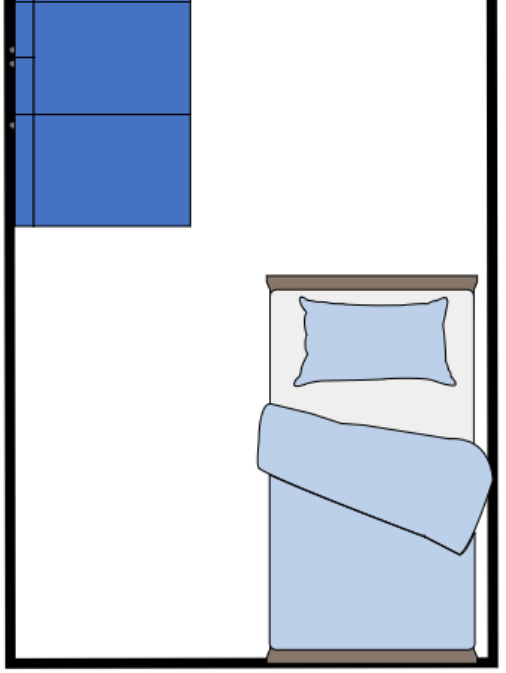
\includegraphics[width=\linewidth]{figures/Liveroom1.png}
        \caption{Guestroom}
        \label{fig:Liveroom1}
    \end{subfigure}
    \hfill
    \begin{subfigure}{0.35\textwidth}
        \centering
        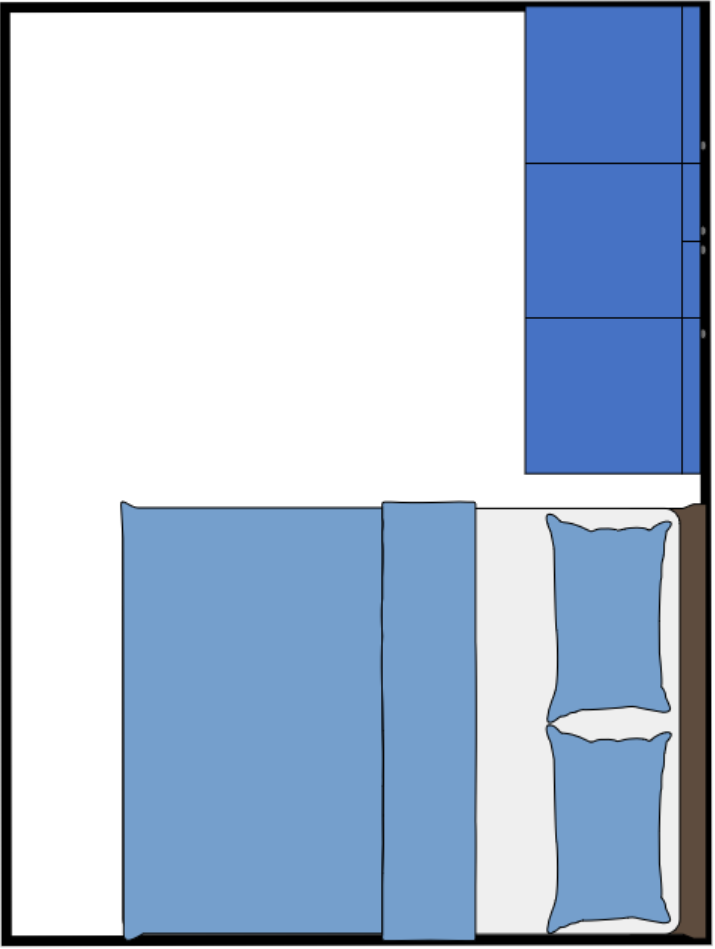
\includegraphics[width=\linewidth]{figures/Liveroom2.png}
        \caption{Bedroom}
        \label{fig:Liveroom2}
    \end{subfigure}
    \hfill
    \begin{subfigure}{0.45\textwidth}
        \centering
        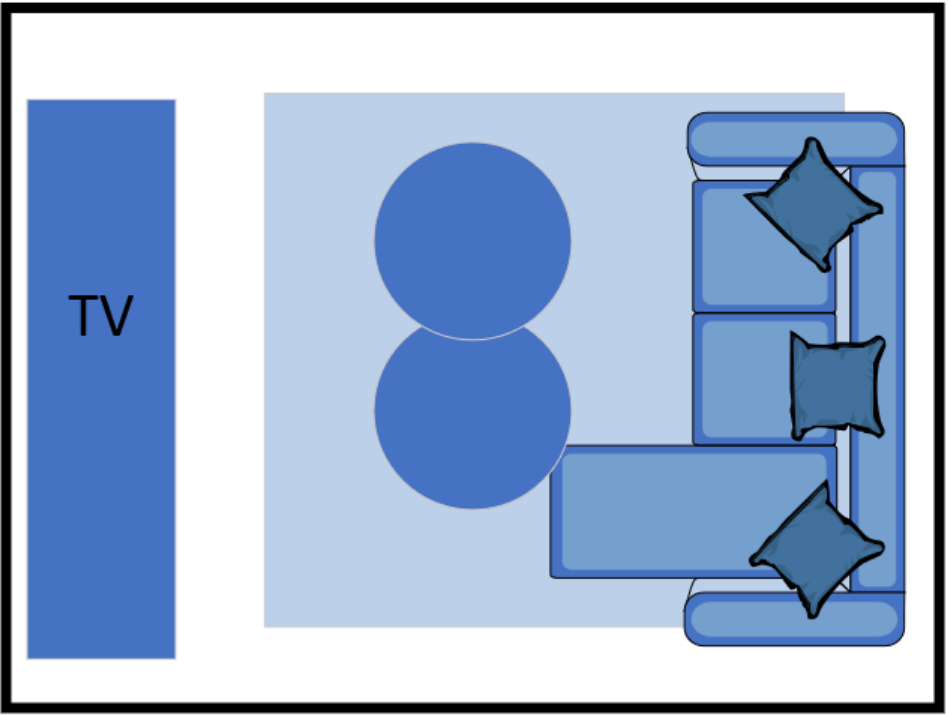
\includegraphics[width=\linewidth]{figures/Liveroom3.png}
        \caption{Living room}
        \label{fig:Liveroom3}
    \end{subfigure}
    
    \caption{Evaluation environments}
    \label{fig:Liveroom}
\end{figure}

For each of the evaluation environments there were connected an additional \gls{IoT} device to the same \gls{SSID} as the Irobot Roomba. These devices generated traffic simulating a real-life smart environment. The additional \gls{IoT} devices and associated evaluation environments are listed below.

\begin{itemize}
    \item \textbf{Guestroom}: IPAD connected
    \item \textbf{Bedroom}: Laptop connected
    \item \textbf{Living room}: Smart phone connected
\end{itemize}

All events were triggered once in each of the evaluation environments. Each event had a 30 minute time window where the event was triggered and finished within. An example of an overall testing schedule is presented in the list below, where the first event is triggered between 08:00 and 08:30. 

\begin{itemize}
    \item First event: between 08:00 and 08:30
    \item Second event: between 08:30 and 09:00
    \item Third event: between 09:00 and 09:30
    \item Fourth event: between 09:30 and 10:00
    \item Fifth event: between 10:00 and 10:30
    \item Sixth event: between 11:30 and 11:00
\end{itemize}

To ensure that the order of events is not affecting the results it was decided by a python script, using the library \textit{random}. Script logic is presented in Figure \ref{fig:Sudo_code_for_event_order_randomize}. This function was executed three times, ensuring that the order of events was random and had minimum influence cross events.

\begin{figure}[H]
    \centering
    \caption{Pseudo code for event order randomize function}
    \label{fig:Sudo_code_for_event_order_randomize}
    \begin{lstlisting}[numbers=left]
         event_list = [scheduled_cleaning, Automated_cleaning, Application_triggered_cleaning, Application_start, Physical_triggered_cleaning, Bin_remove]
         for three rounds do:
              shuffle event_list
              print shuffeled list
    \end{lstlisting}
\end{figure}

The basefilter created during baseline analysis in Chapter \ref{cap:AnalysisandResults} is applied to all the capturing files. This excluded traffic not relevant to the actual event triggered. One additional processing step was included to be able to identify only the relevant corresponding Irobot cloud server. During the restart of the Irobot Roomba it had to request a \gls{DNS} record for \textit{a2uowfjvhio0fa.iot.us-east-1.amazonaws.com} before establishing a \gls{TCP} connection, this \gls{DNS} response was extracted with a python script presented in Appendix \ref{app:DNSex}, an pseudo code is presented in Figure \ref{fig:Sudo_code_for_IP_extraction_from_DNS_response}. This was further identified in Wireshark where the \gls{TCP} hand-shake towards one of the responded \gls{IP} addresses was found. The \gls{IP} observed in the \gls{TCP} handshake was added to the Wireshark filter. All traffic towards \textit{50315.ingest.sentry.io} and \textit{s3.amazoneaws.com} was therefore also excluded, but since only the \gls{DNS} responses are used, all \gls{DNS} traffic is also included in the Wireshark filter and is possible to identify.  

\begin{figure}[H]
    \centering
    \caption{Pseudo code for \gls{IP} extraction from \gls{DNS} response}
    \label{fig:Sudo_code_for_IP_extraction_from_DNS_response}
    \begin{lstlisting}[numbers=left]
        Fuction find_dns_response(event_capture)
          if a2uowfjvhio0fa.iot.us-east-1.amazonaws.com in event_capture
              filter = Responded Ip-addresses and dns
    \end{lstlisting}
 \end{figure}   
 
The new basefilter was applied together with a time filter extracting one capturing file for each 30 minutes, resulting in one event per file. Then event detection algorithm were used on all the event files to evaluate the level of detection in the general smart environment.  

\section{Evaluation Results}

This subsection presents the data processing and rule detection results. First the event order generated by the randomized script is presented. This is followed by the \gls{DNS} extraction and identification of the corresponding Irobot cloud server traffic. Evaluation results are presented and commented. 
Results from the randomize event order function, are presented in Table \ref{tab:evaleventoverview}. The randomization of the event triggering order mitigates the influence cross events. 

\begin{table}[H]
\small
\centering
\caption{Evaluation environments' event triggering order}
\label{tab:evaleventoverview}
\begin{tabular}{|l|l|l|l|}
\hline
\textbf{Order} & \textbf{Guestroom}          & \textbf{Bedroom}          & \textbf{Living room}          \\ \hline
\textbf{1}        & Automated clean                & Application start              & Remove bin                     \\ \hline
\textbf{2}        & App triggered clean            & Scheduled cleaning             & App triggered clean            \\ \hline
\textbf{3}        & Scheduled cleaning             & App triggered clean            & Physical triggered            \\ \hline
\textbf{4}        & Physical triggered            & Physical triggered            & Application start              \\ \hline
\textbf{5}        & Application start              & Automated clean                & Scheduled cleaning             \\ \hline
\textbf{6}        & Bin remove                     & Bin remove                     & Automated cleaning             \\ \hline
\end{tabular}
\end{table}

All capture files got processed by the \gls{DNS} extraction algorithm identifying \gls{DNS} responses for \textit{a2uowfjvhio0fa.iot.us-east-1.amazonaws.com} and extract information about the packet enabling identification in Wireshark. \gls{DNS} responses for packet captures in the three environments are shown in Figure \ref{fig:Evaluation_DNSExtraction}, several \gls{IP} addresses are responded and the Irobot Roomba choose one of these to and establish a \gls{TCP} connection to. 

\begin{figure}[H]
    \centering
    \begin{subfigure}{0.9\textwidth}
        \centering
        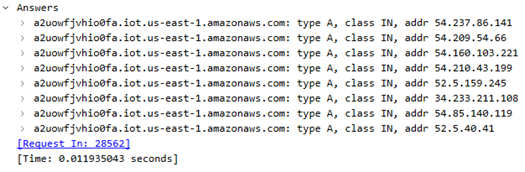
\includegraphics[width=\linewidth]{figures/Evaluation_dns_extraction 1.png}
        \caption{Guestroom DNS extraction}
        \label{fig:Evaluation_DNSextraction_1}
    \end{subfigure}
    \hfill
    \begin{subfigure}{0.9\textwidth}
        \centering
        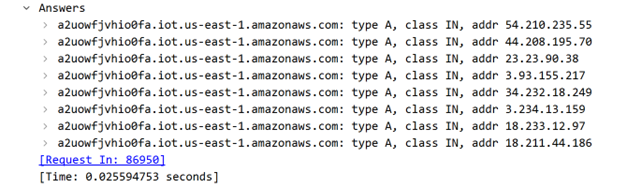
\includegraphics[width=\linewidth]{figures/Evaluation_dns_extraction 2.png}
        \caption{Bedroom DNS extraction}
        \label{fig:Evaluation_DNSextraction_2}
    \end{subfigure}
    \hfill
    \begin{subfigure}{0.9\textwidth}
        \centering
        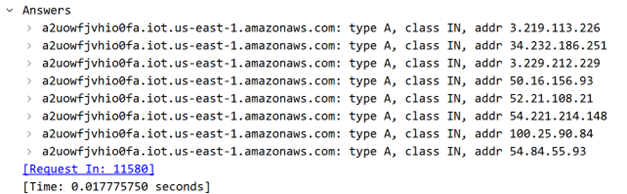
\includegraphics[width=\linewidth]{figures/Evaluation_dns_extraction 3.png}
        \caption{Living room DNS extraction}
        \label{fig:Evaluation_DNSextraction_3}
    \end{subfigure}
    \caption{Evaluation environment DNS extraction}
    \label{fig:Evaluation_DNSExtraction}
\end{figure}

 A \gls{TCP} handshake towards one of the \gls{IP}s in the \gls{DNS} response was identified right after the \gls{DNS} response in Wireshark. The identification of these are presented in Figure \ref{fig:evaluation_corresponding_cloud}. This is a easy way for any attacker to identify corresponding traffic based on \gls{DNS} requests. The used basefilters are listed below, and are identical for all environments except the \gls{IP} address used to identify the Irobot cloud server. 

\begin{itemize}
        \item ((frame.time >= "Apr <day>, 2023 XX:00:00") \&\& (frame.time <= "Apr <day>, 2023 XX:30:00")) AND
        \item (frame.len > 97) AND 
        \item  ((ip.addr == <DNS response IP>) or (dns \&\& ip.dst == 192.168.0.56))
       \item DNS response IPs:  \begin{itemize}
                                \item Guestroom: 54.237.86.141 
                                \item Bedroom: 3.93.155.217 
                                \item Living room: 3.219.113.226 
                            \end{itemize}
\end{itemize}

\begin{figure}[H]
    \centering
    
    \begin{subfigure}{0.80\textwidth}
        \centering
        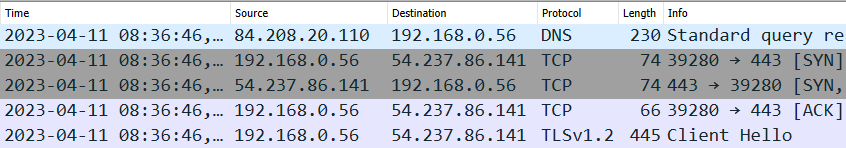
\includegraphics[width=\linewidth]{figures/Evaluation_cloud_detection1.png}
        \caption{Guestroom corresponding Irobot cloud detection}
        \label{fig:Evaluation_coulddetection_1}
    \end{subfigure}
    \hfill
    \begin{subfigure}{0.80\textwidth}
        \centering
        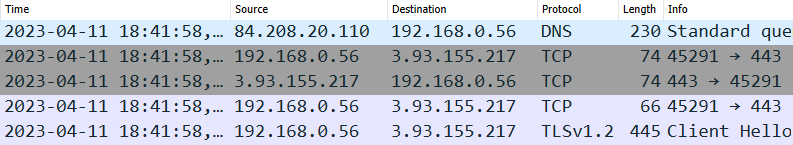
\includegraphics[width=\linewidth]{figures/Evaluation_cloud_detection2.png}
        \caption{Bedroom corresponding Irobot cloud detection}
        \label{fig:Evaluation_clouddetection_2}
    \end{subfigure}
    \hfill
    \begin{subfigure}{0.80\textwidth}
        \centering
        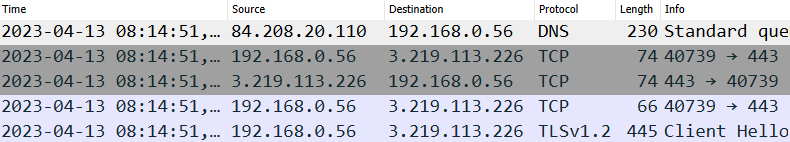
\includegraphics[width=\linewidth]{figures/Evaluation_cloud_detection3.png}
        \caption{Living room corresponding Irobot cloud detection}
        \label{fig:Evaluation_clouddetection_3}
    \end{subfigure}
    
    \caption{Evaluation environments corresponding Irobot cloud detection}
    \label{fig:evaluation_corresponding_cloud}
\end{figure}

All 18 filtered event capturing files were processed by the detection algorithm in Appendix \ref{app:DetectionAlgorithm}. No manual analysis was done to the files before hand and detection results are presented in Table \ref{tab:Evaluation results}. \textit{Scheduled cleaning} and \textit{Physical triggered cleaning} are merged to \textit{Cleaning} but no further signature identification is done. The event is either \textit{Scheduled cleaning} or \textit{Physical triggered cleaning}. 

\begin{table}[H]
\small
\centering
\caption{Evaluation results}
\label{tab:Evaluation results}
\begin{tabular}{|c|c|c|c|c|c|}
\hline
\textbf{Event}        & Auto clean & App clean & Cleaning & App start & Bin removed \\ \hline
\textbf{True positive} & 100\% & 100\%  & 100\% & 100\%  & 0\%         \\ \hline
\textbf{False positive} & 0\%  & 0\%  & 0\% & 0\%  & 66\%         \\ \hline

\end{tabular}
\end{table}

The rules and detection algorithm were able to detect all events, except \textit{Bin remove}, with 100\% accuracy. Cleaning detection resulted in True positive for all cleaning events. \textit{Bin remove} detection gave False negative for all the bin remove events. This might be because the ejection of the bin was executed without causing the Irobot Roomba to lose connection to the charging connectors. The detection algorithm also had False positive identification of \textit{Bin remove} event for 66\% of the events. The bin remove signature is therefore not able to detect bin removal. 




